\documentclass[conference]{IEEEtran}
% \IEEEoverridecommandlockouts % Enable only if a funding footnote is added.

\usepackage{cite}
\usepackage{amsmath,amssymb,amsfonts}
\usepackage{algorithmic}
\usepackage{graphicx}
\usepackage{textcomp}
\usepackage{xcolor}
\usepackage{booktabs}
\usepackage{array}
\usepackage{url}
\usepackage[hidelinks]{hyperref}
\usepackage[section]{placeins}
\usepackage{dblfloatfix}
\usepackage{balance}
\graphicspath{{figures/}}
\urlstyle{same}

\def\BibTeX{{\rm B\kern-.05em{\sc i\kern-.025em b}\kern-.08em
    T\kern-.1667em\lower.7ex\hbox{E}\kern-.125emX}}

\begin{document}

\setlength{\textfloatsep}{9pt plus 1.0pt minus 2.0pt}
\setlength{\floatsep}{8pt plus 1.0pt minus 2.0pt}
\setlength{\intextsep}{8pt plus 1.0pt minus 2.0pt}
\setlength{\abovecaptionskip}{5pt}
\setlength{\belowcaptionskip}{0pt}
\renewcommand{\arraystretch}{1.08}
\clubpenalty=10000
\widowpenalty=10000
\displaywidowpenalty=10000

\title{Low-Light Eye-State Detection Using Subject-Wise Benchmarking and Mixed-Domain Training}

\author{
\IEEEauthorblockN{Your Name}
\IEEEauthorblockA{
\textit{Department / School Name} \\
\textit{College / University Name} \\
City, Country \\
email@example.com}
}

\maketitle

\begin{abstract}
Eye-state classification is a fundamental component of camera-based driver drowsiness monitoring, yet detector performance often degrades under poor illumination. This paper presents a subject-wise study of low-light eye-state detection using a clean Kaggle eye-image dataset reorganized into open and closed classes and evaluated through a controlled synthetic low-light benchmark. A ResNet18-based detector is trained in three settings: clean-only, low-light-only, and mixed clean plus low-light training. To avoid subject leakage, the benchmark is split by subject identity rather than random image-level partitioning. Low-light data are generated from clean eye crops using a moderate synthetic degradation profile named eye\_mid. Experiments are conducted on a balanced 20,000-image benchmark and reported on two held-out 5,000-image test subsets. The clean-only detector achieves strong clean-domain performance but loses low-light robustness, while the low-light-only detector overfits to degraded images and performs poorly on clean images. The mixed detector achieves the best overall trade-off, reaching mean F1 scores of 93.82 on clean data and 93.98 on low-light data, outperforming both alternatives. The novelty of the work lies in a reproducible subject-wise low-light benchmark and a controlled comparison of training-domain strategies rather than in proposing a new backbone architecture. The results show that mixed-domain detector training is a practical and effective strategy for robust low-light eye-state detection.
\end{abstract}

\begin{IEEEkeywords}
drowsiness detection, eye-state classification, low-light vision, transfer learning, ResNet18, subject-wise split
\end{IEEEkeywords}

\section{Introduction}

Driver drowsiness remains a major road-safety concern, and eye-state analysis is one of the most direct visual indicators used in non-intrusive monitoring systems. Recent work has shown that deep learning models can achieve very strong open-eye and closed-eye classification performance for drowsiness-related tasks \cite{hassan2025,florez2024,kim2017}. However, one persistent problem is that performance drops when the input images are captured in low-light conditions, where contrast is reduced and important eyelid boundaries become harder to distinguish.

Recent literature addresses this challenge in different ways. Some studies improve eye-region or drowsiness detection through low-light preprocessing, for example by combining Auto-CLAHE with time-distributed MobileNetV2 \cite{alzami2024}. Others investigate learned low-light enhancement through methods such as Zero-DCE \cite{guo2020}. More broadly, recent computer-vision research has also emphasized that performance under low illumination can benefit from domain adaptation rather than enhancement alone \cite{du2024}. At the same time, recent eye-state and drowsiness studies continue to show that strong backbone architectures, including transfer-learning CNNs and transformers, are effective on open-eye versus closed-eye classification benchmarks \cite{hassan2025}.

Motivated by these observations, this work focuses on a simpler and more controlled question: \emph{how should an eye-state detector be trained so that it remains reliable in low light without sacrificing clean-image performance?} Instead of building a full temporal drowsiness system, we study the detector itself using cropped eye images and compare three training strategies under a subject-wise benchmark:

\begin{itemize}
\item clean-only detector,
\item low-light-only detector,
\item mixed clean plus low-light detector.
\end{itemize}

The main contributions of this paper are as follows:

\begin{itemize}
\item We construct a reproducible subject-wise eye-state benchmark from a public Kaggle eye-image dataset and prevent subject leakage by splitting train, validation, and test sets by subject identity.
\item We generate a matched synthetic low-light benchmark from the clean split using a moderate degradation profile, enabling paired clean-to-low-light robustness analysis on the same labels and subjects.
\item We compare clean-only, low-light-only, and mixed-domain training using the same ResNet18-based detector, which isolates the effect of training-domain design rather than architecture changes.
\item We report the final comparison on two balanced 5,000-image held-out subsets and show that the mixed detector remains stable across both evaluations.
\end{itemize}

The novelty of this paper is therefore \emph{methodological and experimental} rather than architectural. Unlike prior low-light drowsiness approaches that rely mainly on preprocessing, temporal modeling, or enhancement, this work introduces a leak-free evaluation protocol and demonstrates that mixed-domain detector training alone can recover low-light robustness while preserving clean-image performance.

\section{Related Work}

\subsection{Eye-State and Drowsiness Detection}

Eye-state classification has long been used as an important component of drowsiness monitoring, fatigue analysis, and visual attention estimation. Kim \emph{et al.} \cite{kim2017} showed that a deep residual CNN can classify open and closed eyes under varying lighting and resolution conditions better than handcrafted approaches. More recently, Hassan \emph{et al.} \cite{hassan2025} evaluated a wide range of deep architectures, including transfer-learning CNNs and transformers, for open-eye versus closed-eye classification and real-time drowsiness detection, demonstrating that modern deep networks remain highly effective for this task.

\subsection{Low-Light Drowsiness and Eye Analysis}

Low-light conditions present a particularly difficult setting for visual driver monitoring. Alzami \emph{et al.} \cite{alzami2024} addressed this by combining Auto-CLAHE with a time-distributed MobileNetV2 pipeline for eye-region-based drowsiness detection in low light. Their study shows that low-light adaptation is important, but it uses a video-sequence pipeline and contrast enhancement strategy that differs from the detector-only setting considered in this work.

\subsection{Enhancement and Domain Adaptation Under Low Illumination}

Low-light image enhancement methods such as Zero-DCE \cite{guo2020} aim to restore visibility before downstream recognition. These approaches are attractive because they can improve brightness without requiring paired supervision. However, enhancement is not always ideal for narrow-domain inputs such as grayscale eye crops, where visual structure may be altered. Recent work by Du \emph{et al.} \cite{du2024} further supports the broader idea that low-light robustness can come from adaptation across illumination domains rather than relying only on enhancement. This perspective motivates the mixed-domain detector training strategy studied in this paper.

\section{Methodology}

\subsection{Dataset Preparation}

The starting point of the project is a public Kaggle eye-image dataset organized into open-eye and closed-eye classes. For consistency with the training pipeline, the dataset was normalized into the following folder structure:

\begin{itemize}
\item \texttt{raw\_clean/open}
\item \texttt{raw\_clean/closed}
\end{itemize}

Subject identifiers were extracted from the filenames and used to create a leak-free subject-wise split. After dataset auditing and balancing, the final benchmark contained 20,000 images:

\begin{itemize}
\item 10,000 open-eye images,
\item 10,000 closed-eye images.
\end{itemize}

The final usable benchmark contained 16 subjects. These were divided into:

\begin{itemize}
\item 7 training subjects,
\item 4 validation subjects,
\item 5 test subjects.
\end{itemize}

The resulting clean split counts are shown in Table~\ref{tab:split_counts}.

\begin{table}[!t]
\caption{Final subject-wise clean split counts for the curated 20\,000-image benchmark.}
\label{tab:split_counts}
\centering
\footnotesize
\setlength{\tabcolsep}{7pt}
\begin{tabular}{lccc}
\toprule
Split & Open & Closed & Total \\
\midrule
Train & 383 & 383 & 766 \\
Validation & 973 & 973 & 1946 \\
Test & 8644 & 8644 & 17288 \\
\bottomrule
\end{tabular}
\end{table}

The split is intentionally imbalanced across train, validation, and test at the image level because subjects contribute different numbers of images. The key design goal was subject separation rather than equal split size.

\subsection{Synthetic Low-Light Benchmark}

To study robustness under dark conditions while preserving labels and subjects, synthetic low-light versions of the clean images were generated. Several degradation settings were previewed visually, and a moderate setting named \texttt{eye\_mid} was selected for the final experiments. The main parameters were:

\begin{itemize}
\item gamma: 1.75,
\item brightness factor: 0.72,
\item contrast factor: 0.84,
\item black-level shift: 0.02,
\item Gaussian sigma: 1.5,
\item Poisson strength: 0.08.
\end{itemize}

This setting produced visibly darker images while retaining some eye structure, making it suitable for controlled degradation analysis.

\subsection{Detector Architecture}

All final detector experiments use the same backbone so that the comparison isolates the effect of training data rather than architecture changes. The selected detector is a transfer-learning ResNet18 classifier with:

\begin{itemize}
\item input size: $224 \times 224$,
\item standard ResNet18 residual-stage layout: $[2, 2, 2, 2]$ basic blocks,
\item binary output classes: open and closed,
\item single-input raw-image mode,
\item a replaced final classification head for two classes,
\item only the final residual stage unfrozen during transfer learning.
\end{itemize}

ResNet18 was chosen because it offers a good balance between representation strength, training stability, and practical inference cost for a small eye-crop classification problem. Architecturally, it is a residual convolutional network with an initial convolution and pooling stem followed by four residual stages. In the present implementation, the network is adapted as a binary classifier by replacing the final fully connected layer with a two-class prediction head for \emph{open} and \emph{closed} eye states. This choice keeps the model lightweight enough for demonstration and deployment while still benefiting from mature transfer-learning behavior.

\begin{figure}[!t]
\centering
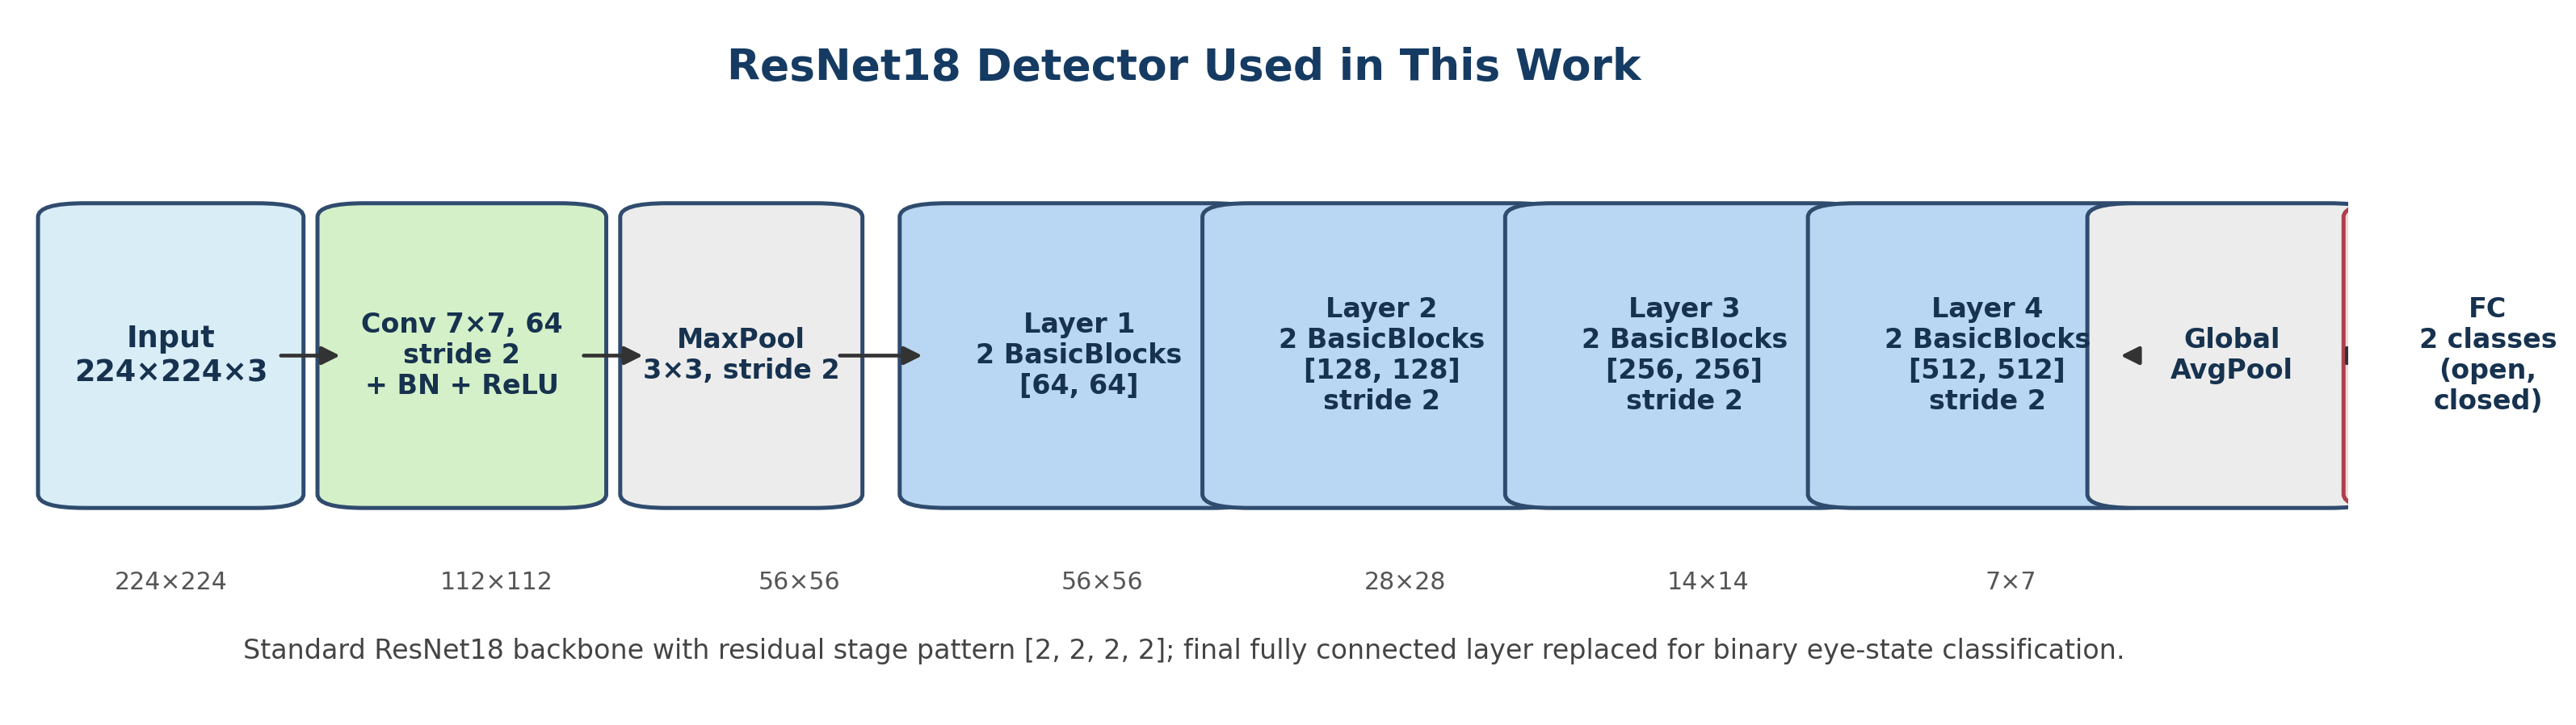
\includegraphics[width=\linewidth]{resnet18_architecture_real.png}
\caption{Architecture of the ResNet18-based detector used in this work. A standard ResNet18 backbone with residual stage pattern $[2, 2, 2, 2]$ is used, and the final fully connected layer is replaced with a two-class output head for \emph{open} and \emph{closed} eye-state prediction.}
\label{fig:resnet18}
\end{figure}

The clean detector was initialized with ImageNet pretrained weights. During adaptation, the classifier head and the final residual stage were allowed to learn the task-specific eye-state features most relevant to the benchmark. The low-light-only and mixed detectors were then initialized from the clean detector checkpoint rather than from ImageNet again. This design keeps the architecture fixed across experiments and makes the comparison primarily a study of \emph{training-domain adaptation}: the clean baseline learns generic eye-state structure, while the later models reuse those learned features and specialize them toward degraded or mixed illumination conditions.

\subsection{Training Strategy}

Three training strategies were compared:

\begin{enumerate}
\item \textbf{Clean detector}: trained on the clean training split only.
\item \textbf{Low-light detector}: fine-tuned only on the low-light training split.
\item \textbf{Mixed detector}: trained on a combined bundle containing both clean and low-light images.
\end{enumerate}

All models were trained using the same general optimization framework:

\begin{itemize}
\item optimizer: AdamW,
\item loss: focal loss with $\gamma = 2.0$,
\item monitor metric: validation F1,
\item threshold tuning objective: validation F1,
\item scheduler: ReduceLROnPlateau,
\item deterministic seed: 42.
\end{itemize}

Data augmentation included resize, random horizontal flip, random rotation, brightness and contrast jitter, optional Gaussian blur, additive Gaussian noise, and ImageNet normalization.

\subsection{Final Experimental Design}

To answer the central research question, the following evaluations were carried out:

\begin{itemize}
\item clean-only detector on clean test images,
\item clean-only detector on low-light test images,
\item low-light-only detector on clean and low-light test images,
\item mixed detector on clean and low-light test images.
\end{itemize}

The final model comparison was repeated on two balanced held-out subsets of 5,000 test images each, sampled with different seeds. Each subset contained 2,500 open-eye and 2,500 closed-eye images.

\begin{figure}[!t]
\centering
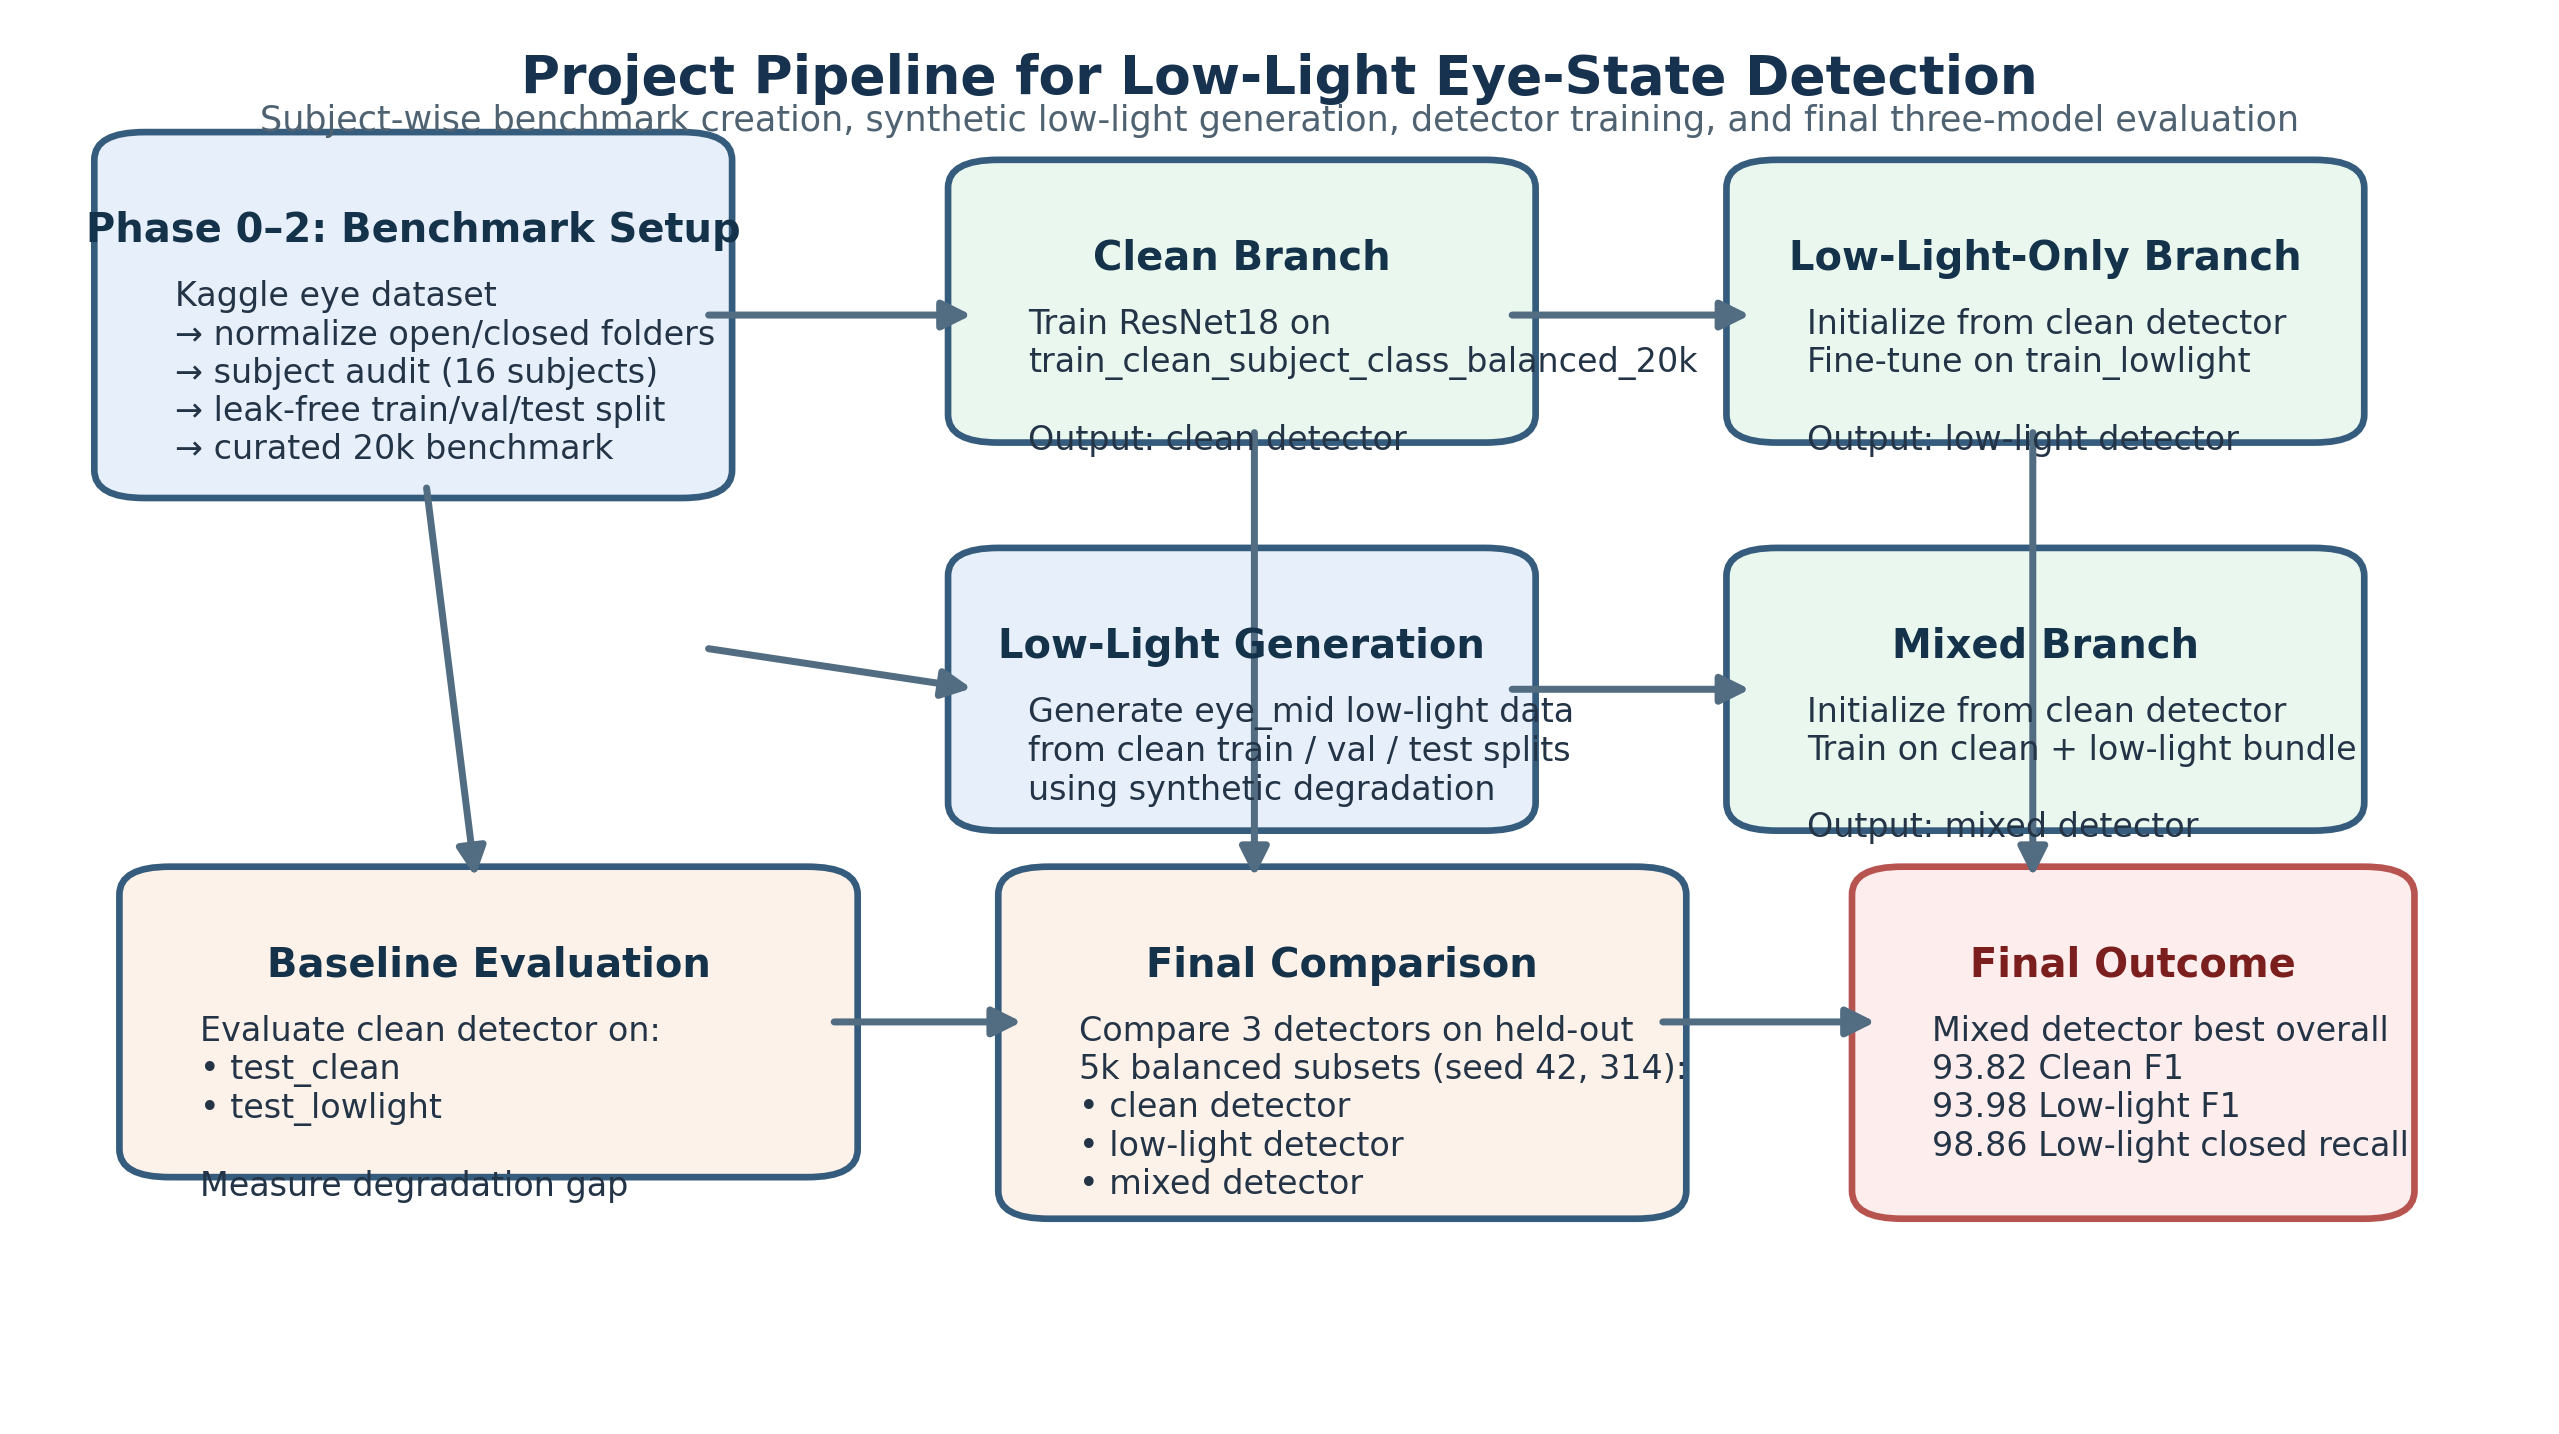
\includegraphics[width=\linewidth]{pipeline_overview_real.png}
\caption{End-to-end project pipeline. The workflow starts with dataset normalization and subject-wise splitting, then branches into clean training, synthetic low-light generation, low-light-only fine-tuning, and mixed-domain training. Final evaluation compares all detectors on held-out balanced subsets.}
\label{fig:pipeline}
\end{figure}

\section{Experimental Setup}

\subsection{Implementation Details}

The benchmark was built and trained in a Colab-based workflow. All eye images, although originally varying from $52 \times 52$ to $209 \times 209$ pixels, were resized to $224 \times 224$ for training and evaluation. The requested batch size was 64, while the effective batch size used in practice was 24.

The main training configurations for the final detectors are summarized in Table~\ref{tab:model_configs}.

\begin{table}[!t]
\caption{Main training settings of the three final detectors.}
\label{tab:model_configs}
\centering
\footnotesize
\setlength{\tabcolsep}{5pt}
\begin{tabular}{>{\raggedright\arraybackslash}p{1.35cm}>{\raggedright\arraybackslash}p{1.55cm}ccc}
\toprule
Model & Training data & Epoch budget & LR & Best threshold \\
\midrule
Clean & Clean only & 15 & $1 \times 10^{-4}$ & 0.70 \\
Low-light & Low-light only & 10 & $3 \times 10^{-5}$ & 0.40 \\
Mixed & Clean + low-light & 12 & $2 \times 10^{-5}$ & 0.50 \\
\bottomrule
\end{tabular}
\end{table}

\subsection{Metrics}

The reported metrics are accuracy, precision, recall, F1 score, and closed-eye recall. Closed-eye recall is especially important because missed closed-eye detections are critical failures in drowsiness monitoring.

\section{Results and Discussion}

\subsection{Quantitative Comparison}

Table~\ref{tab:final_results} summarizes the mean and standard deviation across the two balanced 5\,000-image test subsets.

\begin{table}[!t]
\caption{Compact final comparison across two held-out balanced 5\,000-image subsets.}
\label{tab:final_results}
\centering
\footnotesize
\setlength{\tabcolsep}{3.2pt}
\resizebox{\columnwidth}{!}{%
\begin{tabular}{lcccc}
\toprule
Model & Clean F1 & Low-Light F1 & Closed Recall & Avg. F1 \\
\midrule
Clean detector & 92.86 $\pm$ 0.25 & 88.13 $\pm$ 0.61 & 79.94 $\pm$ 0.76 & 90.50 $\pm$ 0.43 \\
Low-light detector & 69.87 $\pm$ 0.11 & 89.83 $\pm$ 0.06 & 99.18 $\pm$ 0.25 & 79.85 $\pm$ 0.08 \\
Mixed detector & 93.82 $\pm$ 0.11 & 93.98 $\pm$ 0.06 & 98.86 $\pm$ 0.20 & 93.90 $\pm$ 0.08 \\
\bottomrule
\end{tabular}
\par}
\end{table}

Fig.~\ref{fig:results_overview} gives a publication-style visual summary of the same results. It highlights two important points immediately: the clean detector loses low-light performance, especially on closed-eye recall, while the mixed detector remains strong on both clean and low-light domains.

\begin{figure*}[!t]
\centering
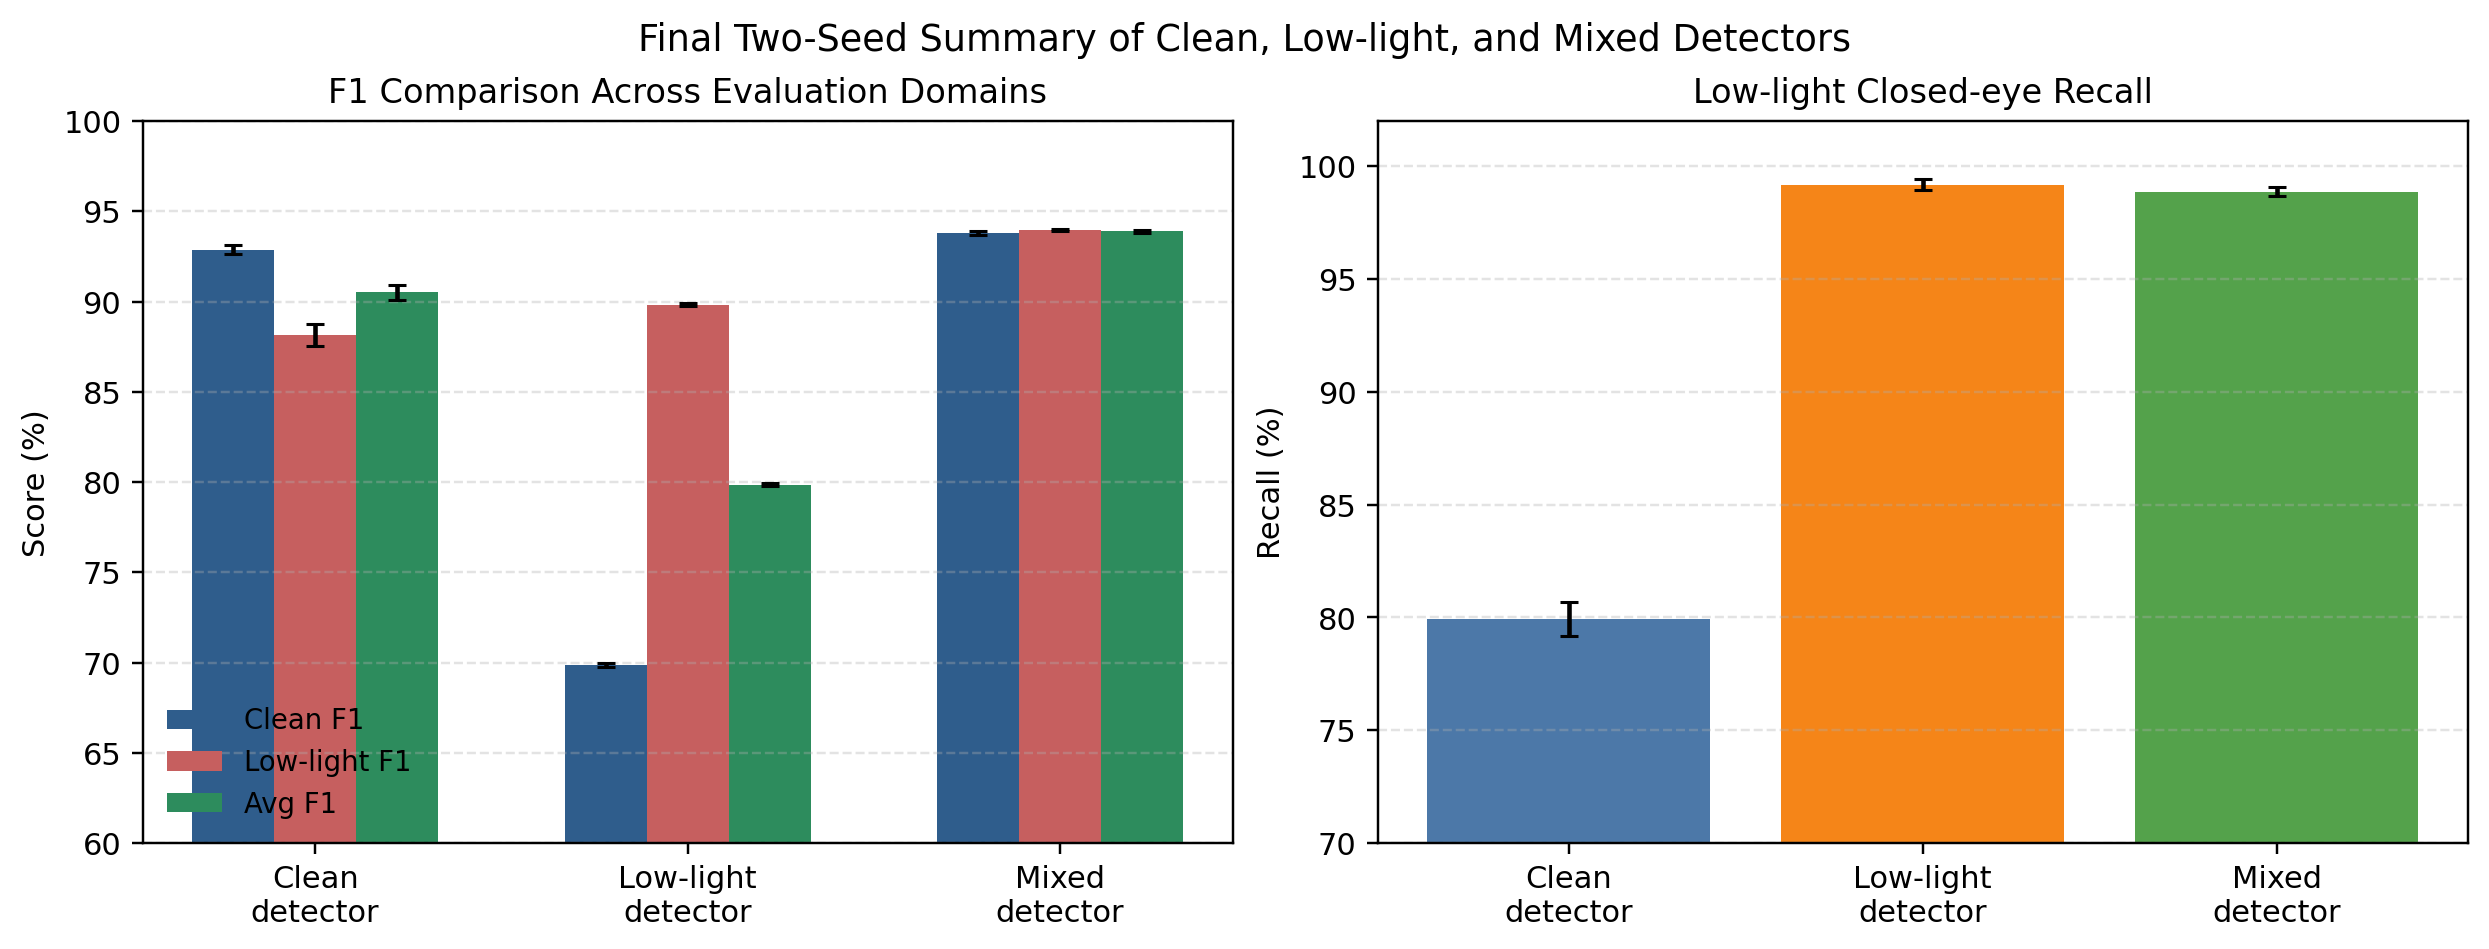
\includegraphics[width=0.96\textwidth]{final_results_overview.png}
\caption{Two-seed summary of the final detector comparison. Left: clean F1, low-light F1, and average F1 for each model. Right: low-light closed-eye recall, which is especially important for safety-oriented drowsiness monitoring.}
\label{fig:results_overview}
\end{figure*}

\begin{figure}[!t]
\centering
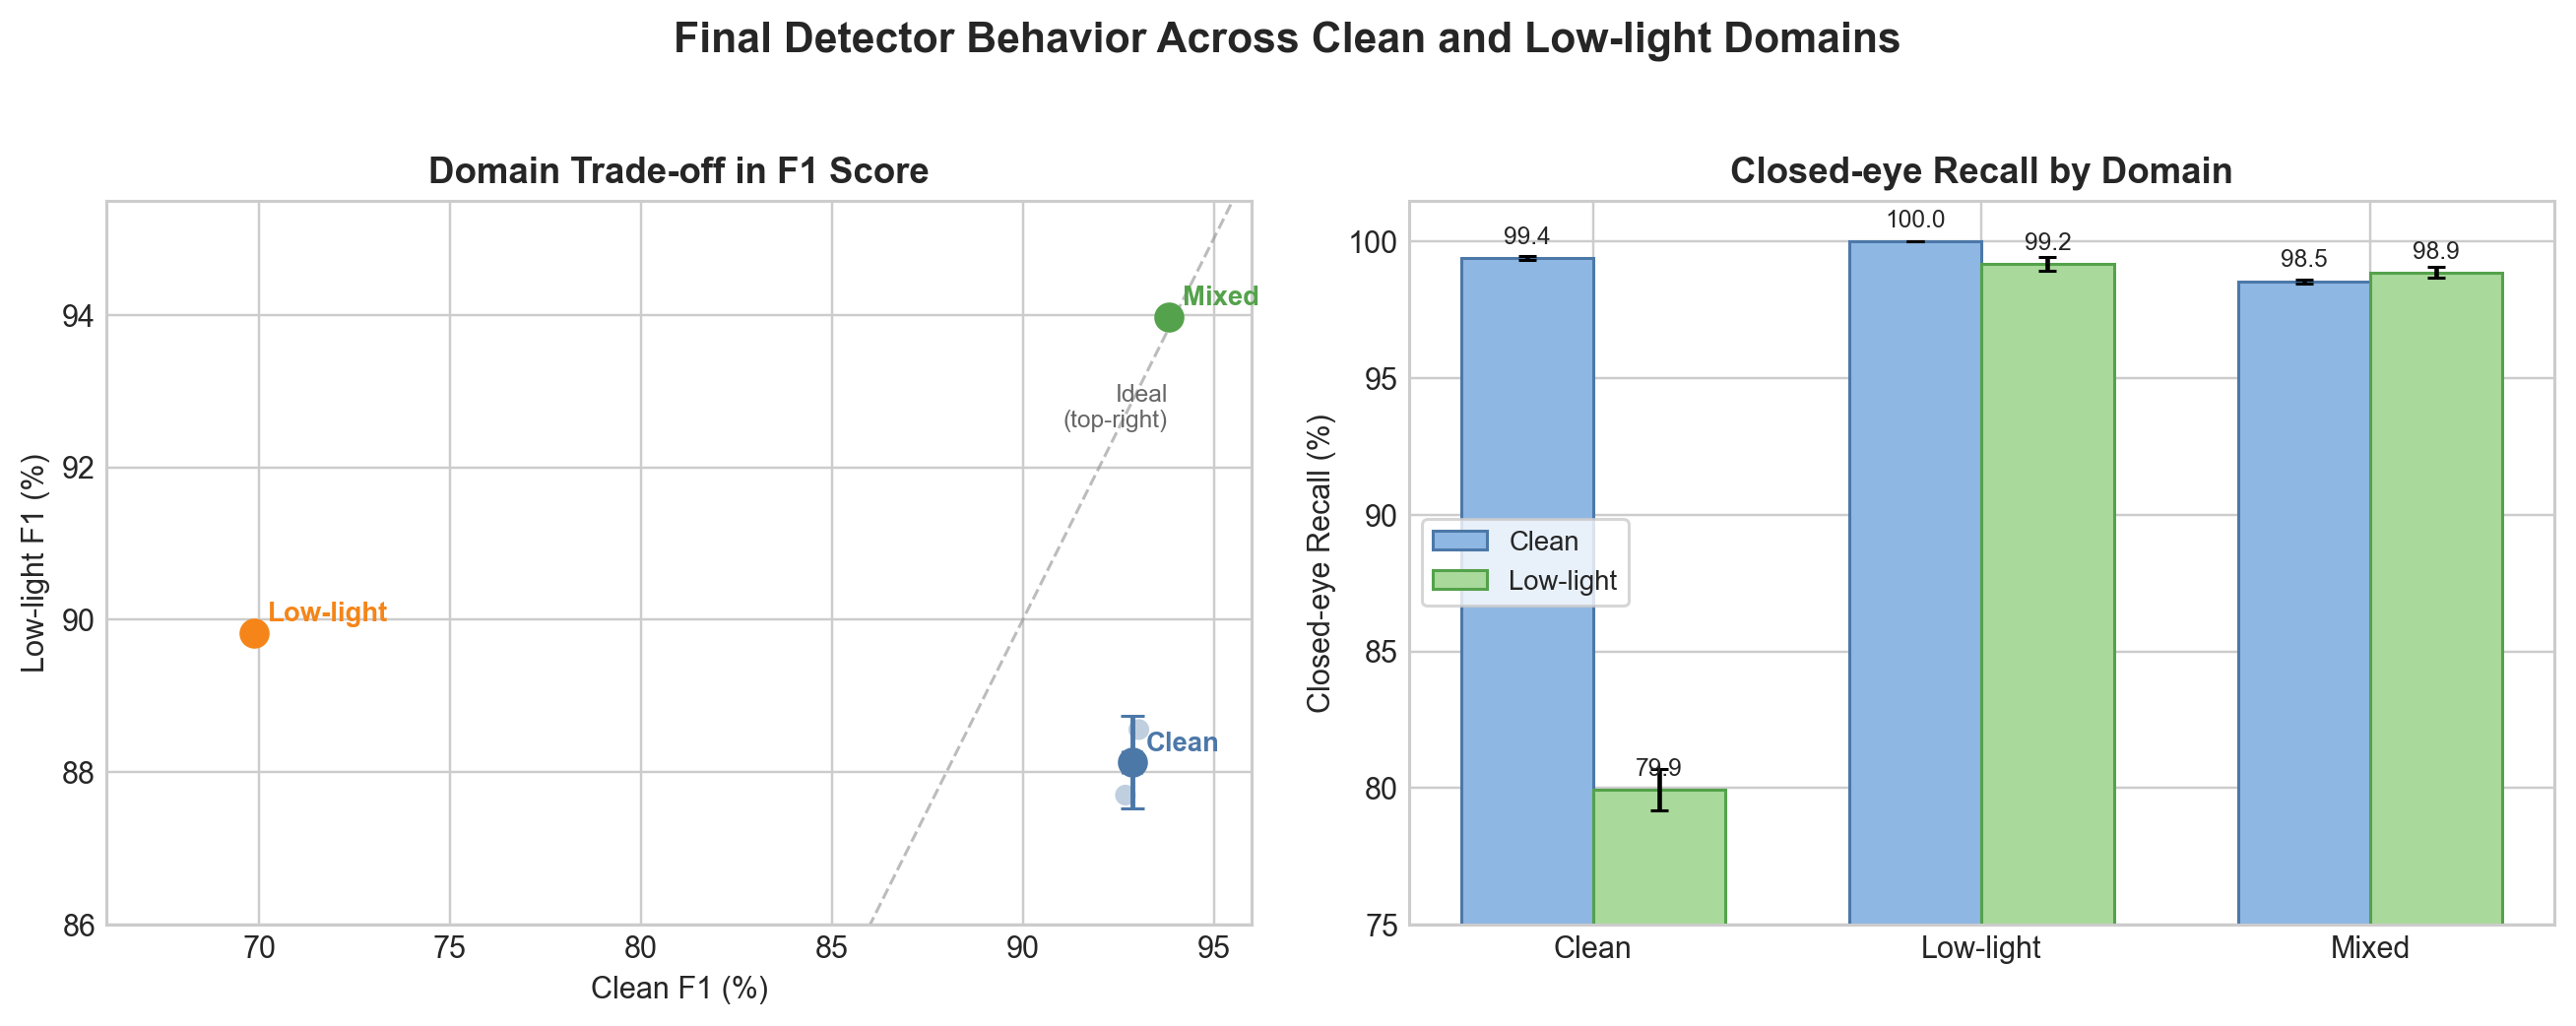
\includegraphics[width=\linewidth]{model_tradeoff_analysis.png}
\caption{Additional view of the final comparison. Left: the clean versus low-light F1 trade-off for each detector, where the desirable region is the top-right corner. Right: closed-eye recall on clean and low-light data, showing that the mixed detector preserves high recall across both domains while the clean baseline drops under low light.}
\label{fig:tradeoff_plot}
\end{figure}

These results support three main conclusions.

First, the clean detector is a strong baseline on well-lit images, but its performance drops in low light. The most important drop is in low-light closed-eye recall, which falls to 79.94. This means that many closed-eye cases are missed when illumination becomes poor.

Second, the low-light-only detector improves low-light robustness, but it severely overfits to the degraded domain. Its clean accuracy falls to 56.88 and its clean F1 falls to 69.87, making it unsuitable as a general-purpose detector.

Third, the mixed detector provides the best trade-off. It improves low-light F1 from 88.13 to 93.98 relative to the clean detector while also slightly improving clean F1 from 92.86 to 93.82. This is the key result of the paper.

Fig.~\ref{fig:tradeoff_plot} makes this trade-off easier to interpret visually. The left panel shows that the low-light-only detector moves toward better low-light F1 but collapses in clean-domain F1, whereas the mixed detector moves toward the desirable top-right corner by improving both. The right panel shows the same conclusion from a safety-oriented perspective: the mixed detector maintains very strong closed-eye recall on clean images and simultaneously recovers low-light closed-eye recall that the clean baseline loses.

To make the trade-off more explicit, Table~\ref{tab:tradeoff_summary} summarizes how each adaptation strategy changes clean-domain and low-light-domain F1 relative to the clean-detector baseline.

\begin{table}[!t]
\caption{Trade-off summary relative to the clean-detector baseline.}
\label{tab:tradeoff_summary}
\centering
\footnotesize
\setlength{\tabcolsep}{4.5pt}
\begin{tabular}{>{\raggedright\arraybackslash}p{1.45cm}cc>{\raggedright\arraybackslash}p{1.35cm}}
\toprule
Model & $\Delta$ Clean F1 & $\Delta$ Low-light F1 & Interpretation \\
\midrule
Clean & 0.00 & 0.00 & Baseline \\
Low-light & $-22.99$ & $+1.70$ & Strong overfitting to degraded images \\
Mixed & $+0.96$ & $+5.85$ & Best trade-off and final model \\
\bottomrule
\end{tabular}
\end{table}

\subsection{Interpretation}

The main practical implication is that low-light robustness should not be treated only as a preprocessing problem. In this project, a Zero-DCE-style enhancement branch was explored in an earlier stage following the broader enhancement literature \cite{guo2020}. However, qualitative inspection showed that enhancement sometimes altered the appearance of grayscale eye crops too strongly. For this reason, the final system focused on detector adaptation instead of enhancement at inference time.

This observation is consistent with the broader low-light detection perspective described by Du \emph{et al.} \cite{du2024}, namely that adaptation across illumination domains can be a powerful route to robustness. In the narrower context of eye-state classification, the present results show that explicitly mixing clean and degraded domains during training is more effective than specializing the detector only to low-light data.

\subsection{Qualitative and Presentation Figures}

\begin{figure*}[!t]
\centering
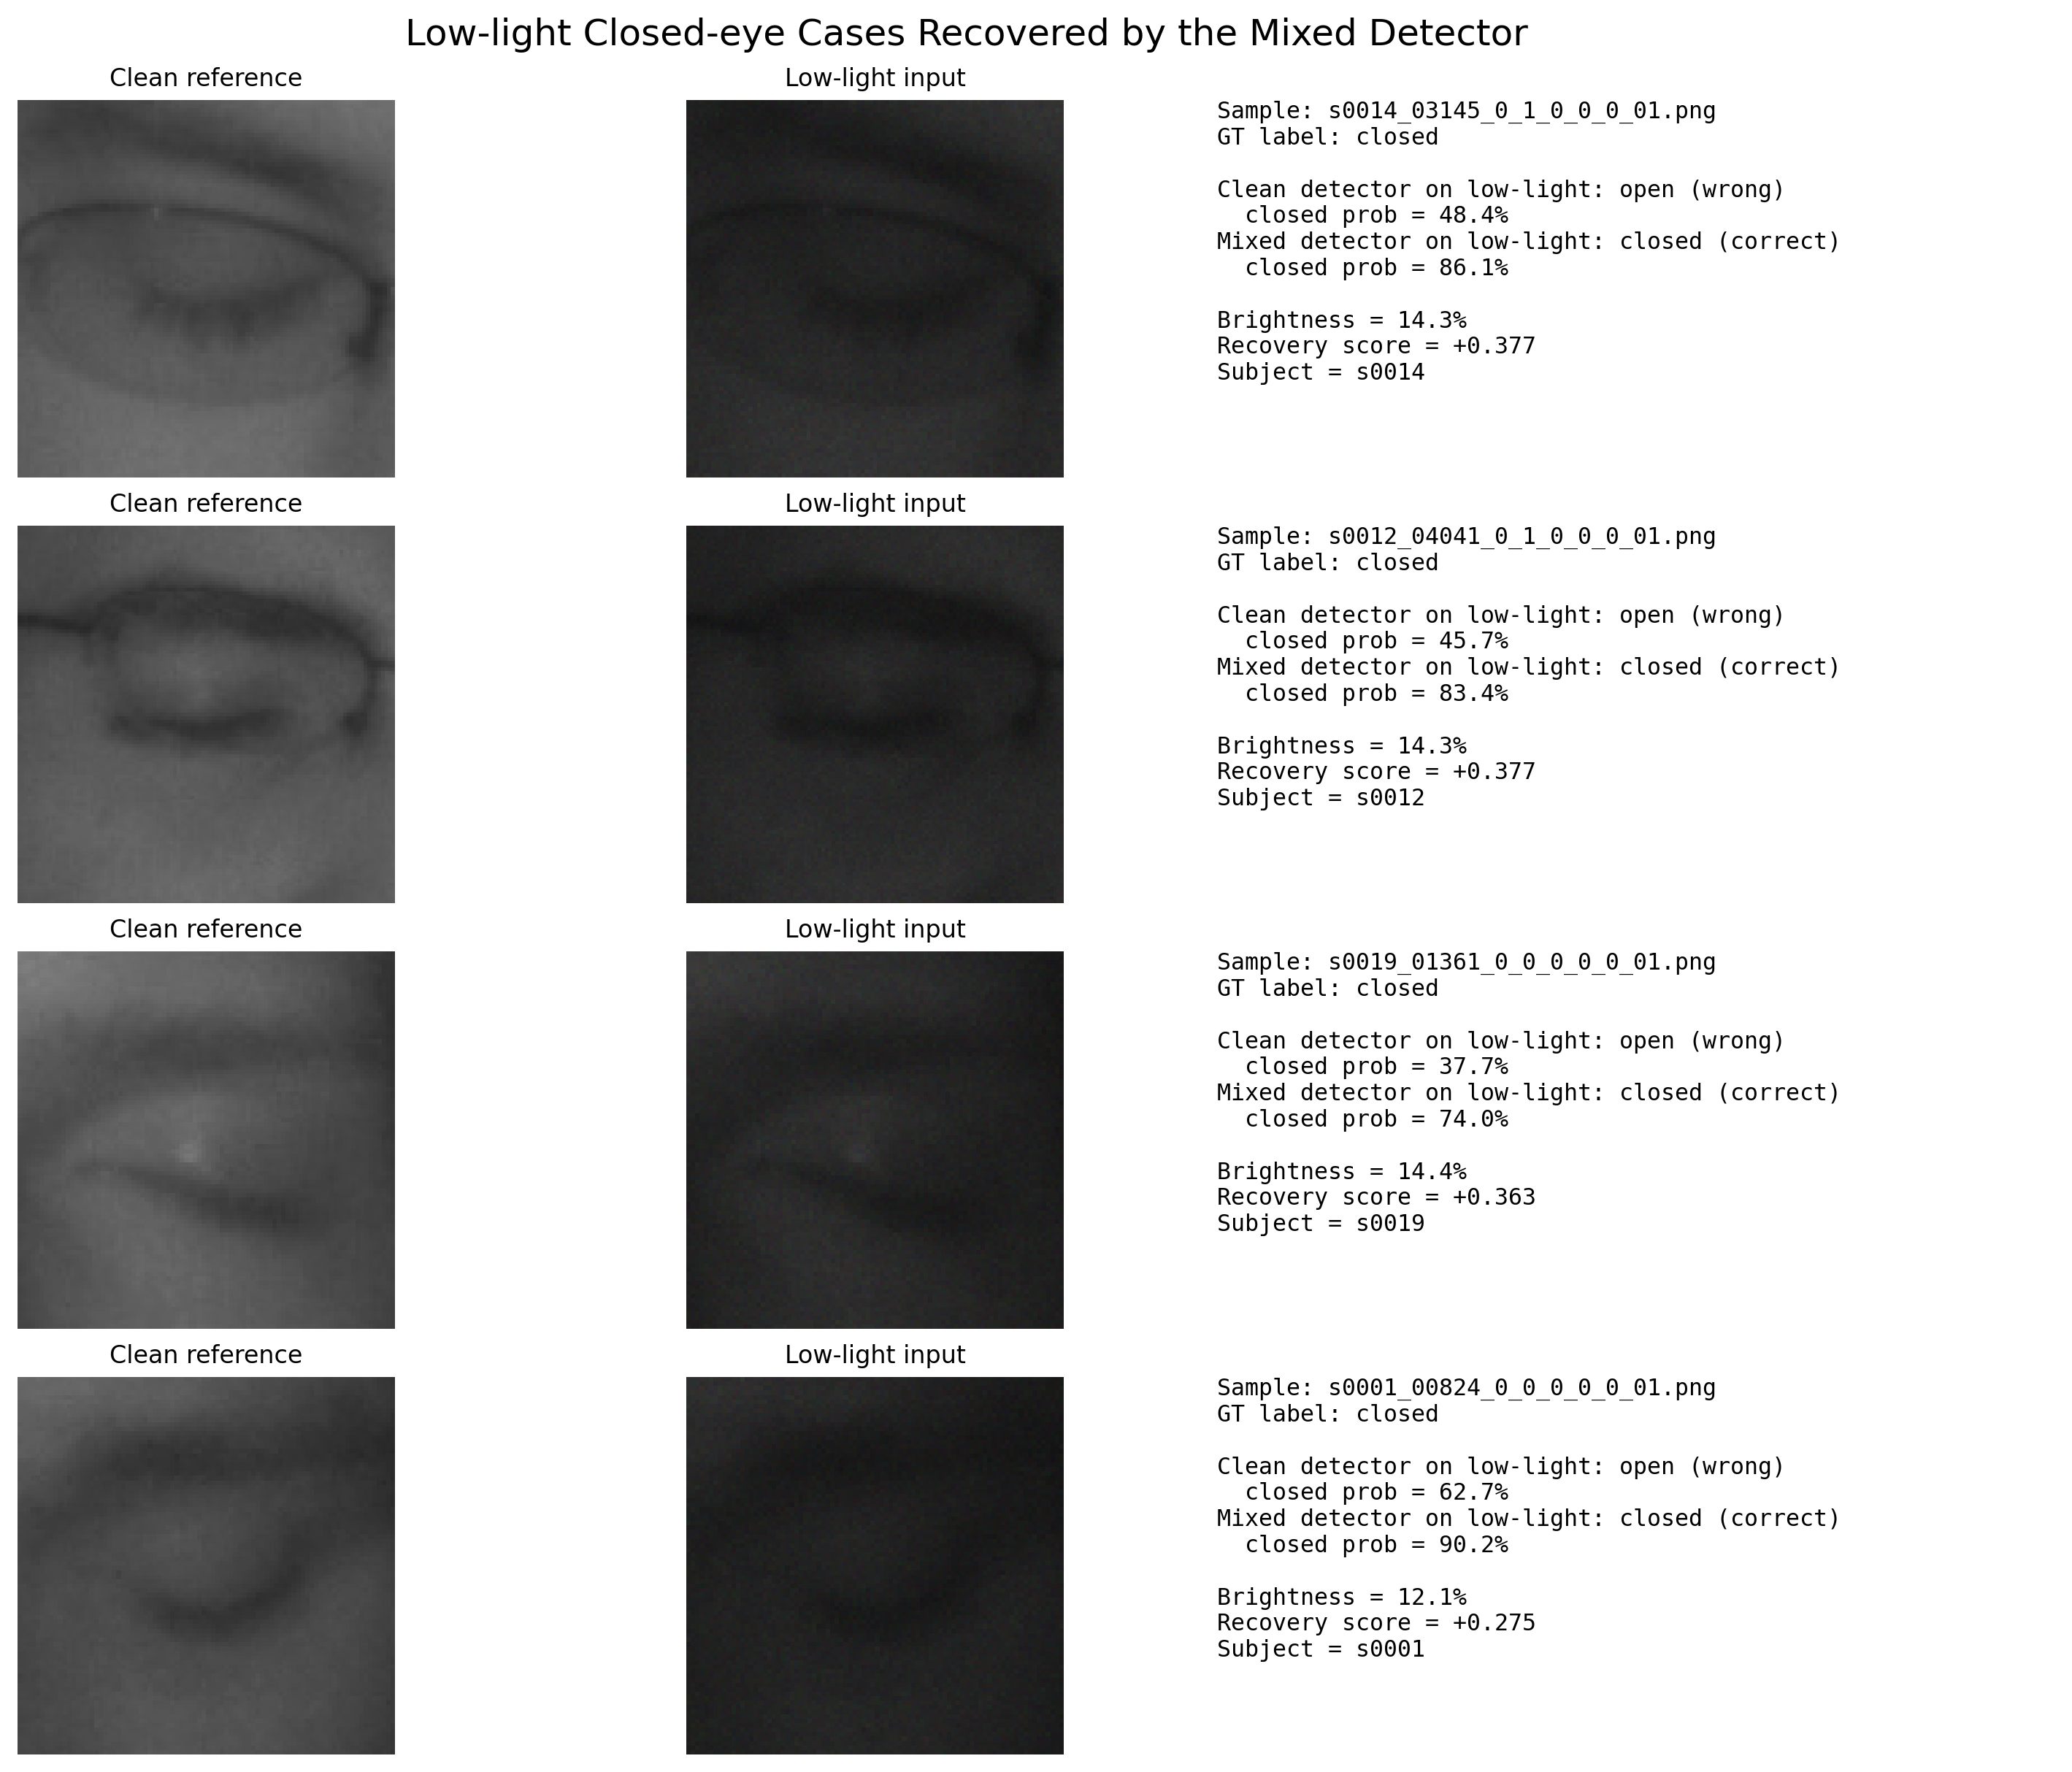
\includegraphics[width=0.96\textwidth]{qualitative_recovery_real.png}
\caption{Real qualitative recovery cases selected from the first held-out 5,000-image subset. Each row shows the clean reference image, the corresponding low-light version, and the predictions made on the low-light input. In all four examples, the clean detector predicts \emph{open} incorrectly, while the mixed detector correctly recovers the \emph{closed} label.}
\label{fig:qualitative}
\end{figure*}

In addition to the manuscript figures, a separate curated demo contact sheet was generated for presentation purposes using eight low-light samples. On this small demonstration set, the clean detector is correct on 6 out of 8 samples, while the mixed detector is correct on all 8 samples. The demo artifact is kept outside the paper body to preserve cleaner IEEE float placement.

\FloatBarrier
\section{Conclusion}

This paper presented a subject-wise study of low-light eye-state detection for drowsiness monitoring using a ResNet18-based transfer-learning detector and a controlled synthetic low-light benchmark. Three training strategies were compared: clean-only, low-light-only, and mixed-domain training. The results show that:

\begin{itemize}
\item clean-only training is not sufficiently robust in low light,
\item low-light-only fine-tuning overfits and damages clean-domain performance,
\item mixed clean plus low-light training gives the best overall detector.
\end{itemize}

The final mixed detector achieved the strongest clean and low-light balance across two held-out 5,000-image test subsets, making it the most practical model for deployment in a low-light eye-state monitoring scenario.

Future work can extend this study by evaluating additional real low-light eye datasets, testing transformer backbones, and incorporating temporal modeling after the single-image detector has been stabilized.

\section*{Acknowledgment}

This work can be updated with the final author affiliation, acknowledgment text, and conference-specific metadata before submission.

\balance
\begin{thebibliography}{00}

\bibitem{hassan2025}
O. F. Hassan, A. F. Ibrahim, A. Gomaa, M. A. Makhlouf, and B. Hafiz, ``Real-time driver drowsiness detection using transformer architectures: a novel deep learning approach,'' \emph{Scientific Reports}, vol. 15, art. no. 17493, 2025, doi: 10.1038/s41598-025-02111-x.

\bibitem{alzami2024}
F. Alzami, M. Naufal, H. Al Azies, S. Winarno, and M. A. Soeleman, ``Time distributed MobileNetV2 with Auto-CLAHE for eye region drowsiness detection in low light conditions,'' \emph{International Journal of Advanced Computer Science and Applications}, vol. 15, no. 11, 2024, doi: 10.14569/IJACSA.2024.0151146.

\bibitem{kim2017}
K. W. Kim, H. G. Hong, G. P. Nam, and K. R. Park, ``A study of deep CNN-based classification of open and closed eyes using a visible light camera sensor,'' \emph{Sensors}, vol. 17, no. 7, art. no. 1534, 2017, doi: 10.3390/s17071534.

\bibitem{guo2020}
C. Guo, C. Li, J. Guo, C. C. Loy, J. Hou, S. Kwong, and R. Cong, ``Zero-reference deep curve estimation for low-light image enhancement,'' in \emph{Proc. IEEE/CVF Conf. Comput. Vis. Pattern Recognit.}, 2020, pp. 1780--1789, doi: 10.1109/CVPR42600.2020.00185.

\bibitem{du2024}
Z. Du, M. Shi, and J. Deng, ``Boosting object detection with zero-shot day-night domain adaptation,'' in \emph{Proc. IEEE/CVF Conf. Comput. Vis. Pattern Recognit.}, 2024, pp. 12666--12676, doi: 10.1109/CVPR52733.2024.01204.

\bibitem{florez2024}
R. Florez, F. Palomino-Quispe, A. B. Alvarez, R. J. Coaquira-Castillo, and J. C. Herrera-Levano, ``A real-time embedded system for driver drowsiness detection based on visual analysis of the eyes and mouth using convolutional neural network and mouth aspect ratio,'' \emph{Sensors}, vol. 24, no. 19, art. no. 6261, 2024, doi: 10.3390/s24196261.

\end{thebibliography}

\end{document}
